\appendix

\chapter{Specification and Progress Report content}
\label{ch:specification-progress-report-content}

\section{Project Requirements}
\label{sec:project-requirements}

The specification document enumerated the set of MoSCoW prioritised \cite{CaseMethodFastTrack} requirements which unambiguously define the project scope. These requirements are replicated below:

\begin{enumerate}
\item
  Select a target mini-app from ECP proxy applications or UK-MAC
  (\textbf{Must have})
\item
  Fuzz test\footnote{an automated testing technique which uses boundary and erroneous test data as inputs, whilst monitoring for resultant undesired behaviour, originally proposed by Miller \textit{et al.} in 1990 \cite{millerEmpiricalStudyReliability1990}\cite{liangFuzzingStateArt2018}} the possible mini-apps for memory safety issues using static analysis tooling \cite{stepanovMemorySanitizerFastDetector2015}
  (\textbf{Should have}, \textit{depends on 1})
\item
  Build tooling for running Rust unit tests on C++ code
  (\textbf{Could have})
\item
  Write unit tests for the original C++ version of the
  mini-app
  (\textbf{Should have}, \textit{depends on 1, (3)})
\item
  Write direct translation of serial version mini-app from C++ to Rust
  (\textbf{Must have}, \textit{depends on 1})
\item
  Modify serial version of translated code to be idiomatic Rust \cite{endlerMreIdiomaticrust2023} 
  (\textbf{Should have}, \textit{depends on 5})
\item
  Equivalence check serial translated code by comparing results of end-to-end tests with original C++ code
  (\textbf{Must have}, \textit{depends on 5}))
\item
  Equivalence check serial translated code by applying passing C++ unit tests to rust code
  (\textbf{Must have}, \textit{depends on 4, 5})
\item
  Equivalence check serial translated code with limited formal verification techniques
  (\textbf{Could have}, \textit{depends on 5})
\item
  Equivalence check serial translated code by comparing generated LLVM IR of the C++ and translated Rust versions
  (\textbf{Could have}, \textit{depends on 5})
\item
  Modify the serial translated code to allow parallel execution
  (\textbf{Must have}, \textit{depends on 5})
\item
  Equivalence check parallel translated code via all previous techniques
  (\textbf{Must have}, \textit{depends on 7, 8, (9), (10), 11})
\item
  Carry out a performance analysis of the serial translated Rust code with the original C++ code
  (\textbf{Must have}, \textit{depends on 5})
\item
  Carry out a performance analysis of the parallel translated Rust code with the original C++ code
  (\textbf{Must have}, \textit{depends on 11})
\item
  Modify the parallel translated code to allow execution across clustered compute resources
  (\textbf{Could have}, \textit{depends on 11})
\item
  Equivalence check clustered translated code via all previous techniques
  (\textbf{Could have}, \textit{depends on 7, 8, (9), (10), 15})
\item
  Carry out a performance analysis of the clustered translated Rust code with the original C++ code
  (\textbf{Could have}, \textit{depends on 15})
\end{enumerate}



\section{Mini-app selection process}
\label{sec:miniapp-selection}

A significant component of early project planning was selecting the mini-app to perform the translation on. Since the translation process would take a significant amount of time, and could be heavily impacted by the properties of the chosen mini-app, it was vital to make an informed selection. The selection process for the mini-app is described below, broadly replicated from the progress report document:

The first objective set out in the specification was ``Select a target mini-app from ECP proxy applications or UK-MAC (\textbf{Must have})'', and all other objectives trivially have a dependency on it.

% Criteria for selection
Between the ECP Proxy Applications \cite{ECPProxyApplications} and UK-MAC \cite{UKMiniAppConsortium}, there were 91 possibilities from which to narrow down. The criteria for initial filtering of the mini-apps was:
\begin{itemize}
    \item The source code for the mini-app must be C++ only (no FORTRAN or Python), in order to conform to the project specification.
    \item The mini-app must not use any High-Performance Computing frameworks, such as Kokkos \cite{KokkosEcosystem} or RAJA \cite{RAJAPortabilitySuite}. This is because they may not have Rust bindings, and the translation of a whole performance framework it out of scope for the project.
    \item The source code for the mini-app must be available as a repository on GitHub, as access to the source code is necessary for the translation process.
\end{itemize}

% Script built for selection
Due to the number of possible applications, a script was written to filter the applications by these criteria. First, the script makes a web request to the page for the application, for example \href{https://proxyapps.exascaleproject.org/app/minimd/}{miniMD}, and parses the unstructured HTML data from this website into a Polars DataFrame \cite{PolarsPolars2023}. If the application has a link to a GitHub repository, it also includes data from a request to the GitHub API \cite{GitHubRESTAPI}. Finally, it uses the scraped data to deselect mini-apps if they don't meet the criteria.

\begin{figure}[h]
    \centering
    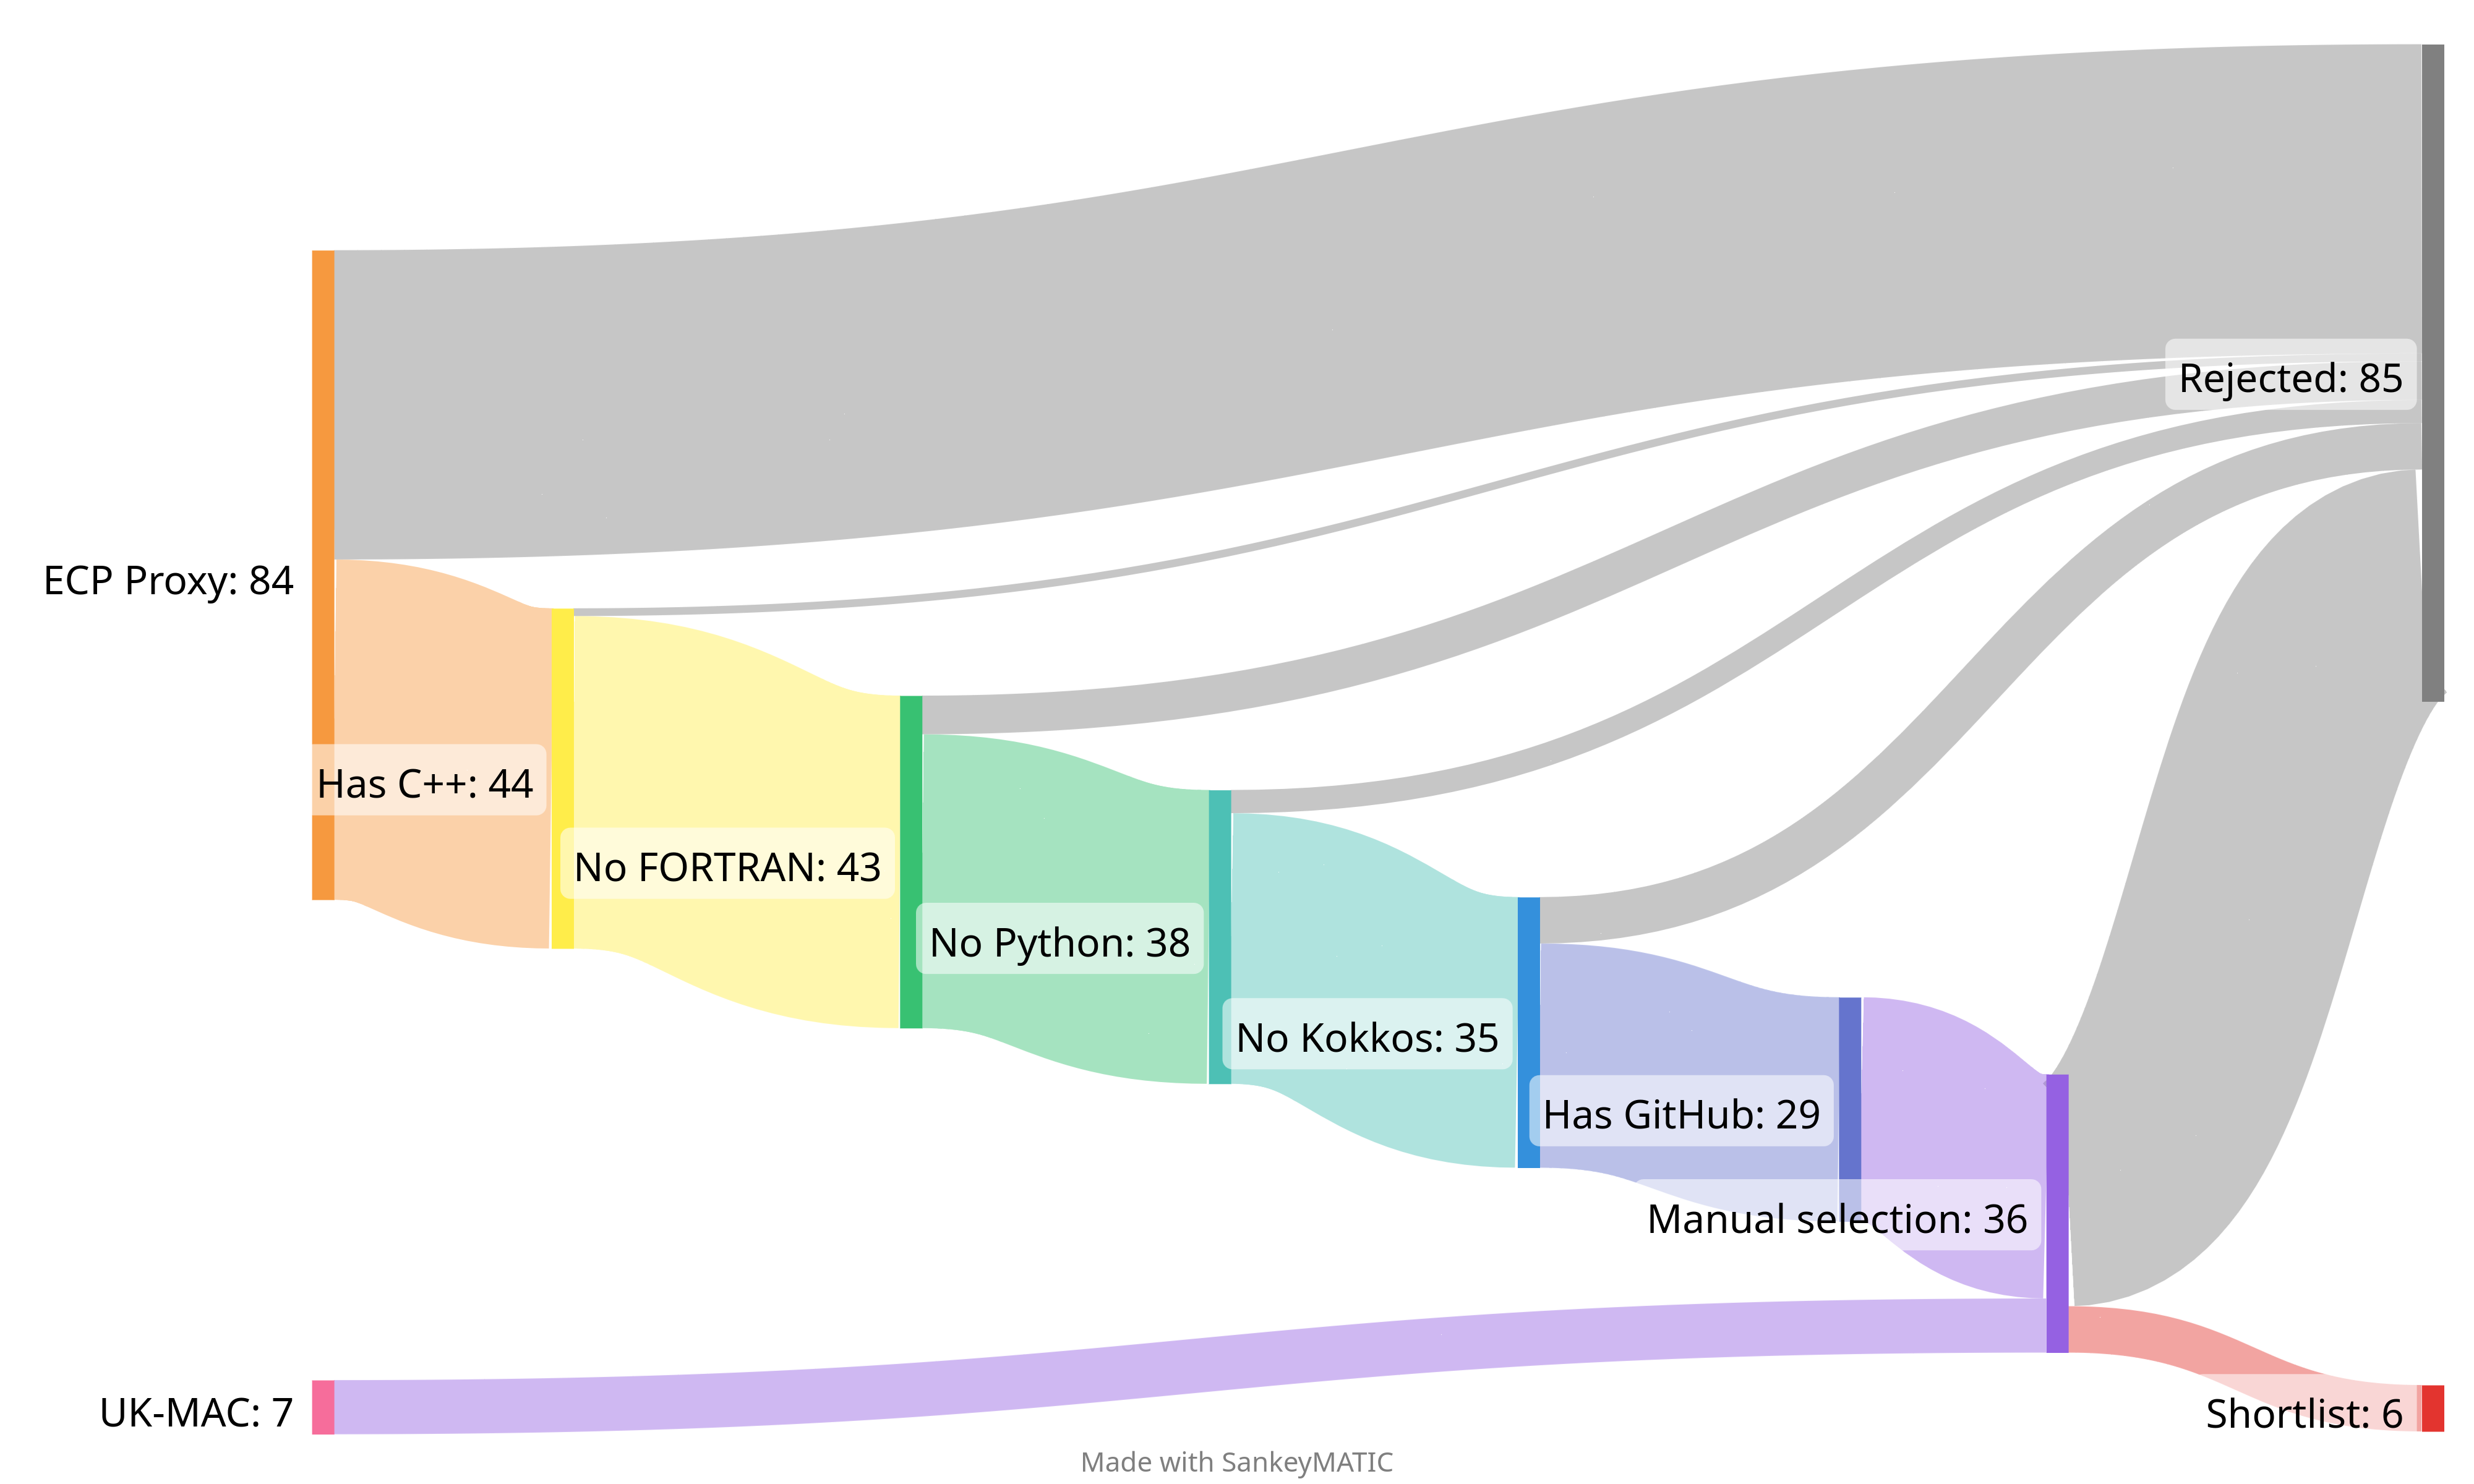
\includegraphics[width=0.75\textwidth]{images/8_appendix/miniapp_sankey.png}
    \caption{Sankey Diagram showing the selection process for the mini-apps, generated by \href{https://sankeymatic.com/build/}{SankeyMatic}.}
    \label{fig:miniapp_sankey}
\end{figure}

After the automated step of the selection process, six of the remaining thirty-six mini-apps were shortlisted, following a discussion with the project supervisor. These shortlisted mini-apps were then manually inspected for the criteria shown in Table \ref{table:miniapps}:

\begin{table}[H]
\centering
    \caption{A table showing the shortlisted mini-apps and their aspects considered when making the final selection.}
    \label{table:miniapps}
    %TC:ignore
    \begin{tabular}{|p{0.14\linewidth}|p{0.125\linewidth}|p{0.12\linewidth}|p{0.1025\linewidth}|p{0.135\linewidth}|p{0.1\linewidth}|}
    \hline
    Name       & Codebase size (lines of code) & Additional dependencies & Tests               & Implemen-tation versions & Memory leaks \\ \hline\hline
    CabanaPIC \cite{ECPcopaCabanaPIC2023} & \cellcolor{green!25}1792 & \cellcolor{red!25}Kokkos & \cellcolor{green!25}Unit and end-to-end & \cellcolor{orange!25}Kokkos only & \cellcolor{red!25}Untested     \\ \hline
    CloverLeaf \cite{CloverLeaf} & \cellcolor{red!25}8045 & \cellcolor{green!25}None & \cellcolor{orange!25}End-to-end & \cellcolor{green!25}Many & \cellcolor{orange!25}None         \\ \hline
    HPCCG \cite{herouxHPCCGSolverPackage2007} & \cellcolor{green!25}1542 & \cellcolor{green!25}None & \cellcolor{orange!25}End-to-end & \cellcolor{orange!25}OpenMP and MPI only & \cellcolor{green!25}375 kB       \\ \hline
    MiniMD \cite{osti_1231191} & \cellcolor{orange!25}4082 & \cellcolor{green!25}None & \cellcolor{orange!25}End-to-end & \cellcolor{green!25}Many & \cellcolor{green!25}5.82 MB      \\ \hline
    TeaLeaf \cite{TeaLeaf2023} & \cellcolor{orange!25}2580 & \cellcolor{green!25}None & \cellcolor{orange!25}End-to-end & \cellcolor{green!25}Many & \cellcolor{orange!25}None         \\ \hline
    VPFFT++ \cite{VPFFT2023}   & \cellcolor{orange!25}3384 & \cellcolor{red!25}Eigen, FFTW & \cellcolor{orange!25}Unit & \cellcolor{orange!25}MPI only & \cellcolor{red!25}Untested     \\ \hline
    \end{tabular}
    %TC:endignore
\end{table}

These mini-apps were manually inspected for the size and quality of their codebase (smaller and higher quality is better, assessed using the \texttt{sloccount} \cite{SLOCCount} and the \texttt{clang-tidy} linter \cite{ClangTidyExtraClang}), whether they had unit tests, whether they had multiple versions for serial/parallel, historical prominence, and whether they had any memory leaks using \texttt{valgrind} \cite{ValgrindHome}.

\begin{code}
    \begin{verbatim}
==33790== 
==33790== HEAP SUMMARY:
==33790==     in use at exit: 5,875,096 bytes in 10 blocks
==33790==   total heap usage: 149 allocs, 139 frees, 6,348,737 bytes allocated
==33790== 
[snip]
==33790== 
==33790== LEAK SUMMARY:
==33790==    definitely lost: 375,096 bytes in 4 blocks
==33790==    indirectly lost: 5,500,000 bytes in 6 blocks
==33790==      possibly lost: 0 bytes in 0 blocks
==33790==    still reachable: 0 bytes in 0 blocks
==33790==         suppressed: 0 bytes in 0 blocks
==33790== 
==33790== For lists of detected and suppressed errors, rerun with: -s
==33790== ERROR SUMMARY: 4 errors from 4 contexts (suppressed: 0 from 0)
    \end{verbatim}
    \caption{Snippet of the output of running \texttt{valgrind} on the HPCCG mini-app, with over 375kB directly lost over a test run with mesh size $25 \times 25 \times 25$.}
    \label{fig:minimdValgrindOutput}
\end{code}

Interestingly, some shortlisted mini-apps, including HPCCG, MiniMD, and TeaLeaf, leak memory -- as shown in the Figure \ref{fig:minimdValgrindOutput}. This is emblematic of one of the main drawbacks of C++ -- the ease with which it is to do manual memory management wrong. In contrast, Rust is designed to abstract away memory management from the programmer, instead focussing on the resultant properties of data ownership and lifetimes.

After a manual comparison process on the aspects shown above, the decision was made to select the HPCCG mini-app for the translation process, due to its: small, high quality codebase and simple build system; absence of additional required dependencies; existing implementations for both OpenMP and MPI; and the presence of memory leaks.

\section{Risk matrix}
\label{sec:risk-matrix-appendix}

% When generating the Risk Matrix for the specification, some possible risks were excluded, such as personal computer failure. However, this was experienced multiple times during the project

\begin{table}[ht]
\begin{adjustwidth}{-3em}{-3em}
    \centering
    \caption{The proposed Risk Matrix for the project, from the project specification.}
    \label{tab:risk_matrix}
    %TC:ignore
    \begin{tabular}{|p{0.2\linewidth}|p{0.25\linewidth}|p{0.065\linewidth}|p{0.085\linewidth}|p{0.055\linewidth}|p{0.24\linewidth}|} \hline
         \textbf{Risk} & \textbf{Cause of risk} & \textbf{Bad- ness} & \textbf{Likeli- hood} & \textbf{Score} & \textbf{Mitigation strategy}\\ \hline\hline
         Major upheaval of the Rust language&  The Rust Foundation making a controversial decision \cite{AmNoLonger2023} \cite{AddRFCGovernance} \cite{TelemetryGoToolchain}&  4&  1&  \cellcolor{green!25}4 & Use a previous edition of Rust via \texttt{rustup}\\ \hline 
         Data structure for selected \acrshort{mini-app} cannot be recreated under Rust's memory safety
  constraints&  Some data structures cannot be represented with Rust's ownership model, such as doubly linked lists \cite{leeBuildingMemorysafeNetwork2017}&  5&  6&  \cellcolor{red!25}30& Create a safe API around the required unsafe data structure\\ \hline 
         Compute resources become busy slowing development and testing&    Towards the end of term two, many students use \texttt{kudu} for coursework and dissertations&  2&  8&  \cellcolor{orange!25}16& Use a different compute resource, for example if \texttt{kudu} is busy use SCRTP or local machines\\ \hline 
         Unable to install Rust on compute resources&  Some compute resources may have restrictive permissions for users&  9&  3&  \cellcolor{red!25}27& Install only for a single user, or leverage containerisation to avoid installation issues\\ \hline 
 Loss of access to IBM computer resources or mentor and connections& Internal changes to IBM unrelated to the project& 4& 1& \cellcolor{green!25}4 &Whilst the IBM resources are nice to have, none of them are essential to the project, so can just continue without them\\ \hline
    \end{tabular}
    %TC:endignore
    \end{adjustwidth}
\end{table}

\section{HPCCG sparse matrix format}
\label{sec:hpccg-sparse-matrix-appendix}

The following example describes how HPCCG uses a pointer-based variant of the compressed row storage format to represent sparse matrices, such as the one shown in Equation \ref{eq:exampleMatrix}.

\begin{align}
    \begin{pmatrix}
        0 & 1 & 0 & 2 \\
        0 & 0 & 5 & 0 \\
        0 & 4 & 6 & 0 \\
        3 & 0 & 0 & 0
    \end{pmatrix}
    \label{eq:exampleMatrix}
\end{align}

A sparse matrix can then be represented as two nested lists -- one containing the non-zero values in each row, and the other the indices of those non-zero values in that row. This means the sparse matrix in (\ref{eq:exampleMatrix}) can be written as:

\begin{verbatim}
list_of_vals = [   [1, 2]  ,  [5]  ,  [4, 6]  ,  [3]   ]
list_of_inds = [   [1, 3]  ,  [2]  ,  [1, 2]  ,  [0]   ]
\end{verbatim}
% \begin{align}
%     \verb!list_of_vals = [   [1, 2]  ,  [5]  ,  [4, 6]  ,  [3]   ]! \\
%     \verb!list_of_inds = [   [1, 3]  ,  [2]  ,  [1, 2]  ,  [0]   ]!
%     \label{eq:exampleMatrixRepr}
% \end{align}

This structure uses much less memory, but has the drawback that the inner lists for each row are of variable length, making the outer list non-homogenous. HPCCG's data structure is a flattening of the above structure to use single-dimensional arrays rather than nested ones for \texttt{list\_of\_vals} and \texttt{list\_of\_inds}. This then requires a mechanism to distinguish rows, so it uses auxiliary data structures for the lengths of each row (an array of integers called \texttt{nnz\_in\_row}), along with pointers to the start of each row in the values and indices arrays (two arrays of pointers called \texttt{ptr\_to\_vals\_in\_row} and \texttt{ptr\_to\_inds\_in\_row} respectively). Finally, the number of rows (an integer called \texttt{total\_nrow}) is also needed. Hence, HPCCG would represent the sparse matrix in (\ref{eq:exampleMatrix}) as follows:

\begin{verbatim}
total_nrow          = 4
nnz_in_row          = [ 2 ,     1 , 2 ,     1 ]
list_of_vals        = [ 1 , 2 , 5 , 4 , 6 , 3 ]
ptr_to_vals_in_row  = [ ↑ ,     ↑ , ↑,      ↑ ]
list_of_inds        = [ 1 , 3 , 2 , 1 , 2 , 0 ]
ptr_to_inds_in_row  = [ ↑ ,     ↑ , ↑,      ↑ ]
\end{verbatim}

To traverse the values in a row $i$ of this data structure, first retrieve the pointer to the starting point in the list of values from \texttt{ptr\_to\_vals\_in\_row[i]}. Then, traverse through the list of values for the number of non-zeroes, \texttt{nnz\_in\_row[i]}. This same process applies to traversing indices in a row.

This data structure provides significant performance improvements over a full matrix representation for the sparse matrix-vector multiplication operation. This is because it minimises both the memory bandwidth and arithmetic operations required, by omitting the zero-values which would not contribute to the product.









\chapter{HPC MultiBench}
\label{ch:tooling-appendix}

\section{Replication study YAML}
\label{sec:tooling-replication-yaml}

The YAML file which fully defines the replication study using the HPC MultiBench tool of Moran and Bull's paper ``Emerging Technologies, Rust in HPC'' \cite{moranEmergingTechnologiesRust2023} can be seen in Listing \ref{listing:replication-study-yaml-file} below:

\begin{code}
    \begin{minted}{yaml}
run_configurations:
  "cpp-serial":
    sbatch_config:
      "nodes": 1
      "ntasks-per-node": 1
      "cpus-per-task": 1
      "exclusive": "mcs"
      "mem": 60000
    module_loads: []
    environment_variables: {}
    directory: "./generated_results/eurocc_cfd-kudu-results/eurocc_cfd/C-SER"
    build_commands:
      - "make"
    run_command: "./cfd"

  "fortran-serial":
    sbatch_config:
      "nodes": 1
      "ntasks-per-node": 1
      "cpus-per-task": 1
      "exclusive": "mcs"
      "mem": 60000
    module_loads: []
    environment_variables: {}
    directory: "./generated_results/eurocc_cfd-kudu-results/eurocc_cfd/F-SER"
    build_commands:
      - "make"
    run_command: "./cfd"

  "rust-serial":
    sbatch_config:
      "nodes": 1
      "ntasks-per-node": 1
      "cpus-per-task": 1
      "exclusive": "mcs"
      "mem": 60000
    module_loads: []
    environment_variables: {}
    directory: "./generated_results/eurocc_cfd-kudu-results/eurocc_cfd/cfd"
    build_commands:
      - "cargo build --release"
    run_command: "./target/release/cfd"

  "cpp-openmp":
    sbatch_config:
      "nodes": 1
      "ntasks-per-node": 1
      "cpus-per-task": 32
      "exclusive": "mcs"
      "mem": 60000
    module_loads: []
    environment_variables: {}
    directory: "./generated_results/eurocc_cfd-kudu-results/eurocc_cfd/C-OMP"
    build_commands:
      - "make"
    run_command: "./cfd"

  "fortran-openmp":
    sbatch_config:
      "nodes": 1
      "ntasks-per-node": 1
      "cpus-per-task": 32
      "exclusive": "mcs"
      "mem": 60000
    module_loads: []
    environment_variables: {}
    directory: "./generated_results/eurocc_cfd-kudu-results/eurocc_cfd/F-OMP"
    build_commands:
      - "make"
    run_command: "./cfd"

  "rust-rayon":
    sbatch_config:
      "nodes": 1
      "ntasks-per-node": 1
      "cpus-per-task": 32
      "exclusive": "mcs"
      "mem": 60000
    module_loads: []
    environment_variables: {}
    directory: "./generated_results/eurocc_cfd-kudu-results/eurocc_cfd/cfd_rayon"
    build_commands:
      - "cargo build --release"
    run_command: "./target/release/cfd"

benches:
  "serial":
    run_configurations:
      - "rust-serial"
      - "cpp-serial"
      - "fortran-serial"
    reruns:
      number: 5
      unaggregatable_metrics:
        - "Scale factor"
        - "Iterations"
        - "Grid x size"
        - "Problem size"
    matrix:
      args:
        - "1 5000"
        - "2 5000"
        - "4 5000"
        - "8 5000"
        - "16 5000"
        - "32 5000"
        - "64 5000"
        - "128 5000"
    analysis:
      metrics:
        "Scale factor": "Scale [F|f]actor =\\s+(\\d+),"
        "Iterations": ", iterations =\\s+(\\d+)"
        "Grid x size": "Running CFD on\\s+(\\d+) x\\s+\\d+ grid"
        "Problem size": "=== RUN INSTANTIATION ===\n\\{.*args: (\\d+) .*\\}"
        "Total time (s)": "Time for\\s+\\d+ iterations was\\s+([\\d\\.eE\\-+]+)\\s+seconds"
        "Iteration time (s)": "Each i?n?d?i?v?i?d?u?a?l? ?iteration took\\s+([\\d\\.eE\\-+]+)\\s+seconds"
      derived_metrics:
        "Iterations per second": "1 / metrics['Iteration time (s)']"
        "Execution time relative to C++": "metrics['Iteration time (s)'] / _corresponding_metrics['cpp-serial']['Iteration time (s)']"
      line_plots:
        - title: "Serial Implementation Comparison"
          x: "Problem size"
          y: "Total time (s)"
          y_log: True
        - title: "Relative execution times to C++"
          x: "Problem size"
          y: "Execution time relative to C++"
          y_lim: [0.6, 2.2]

  "parallel":
    run_configurations:
      - "rust-rayon"
      - "cpp-openmp"
      - "fortran-openmp"
    reruns:
      number: 5
      unaggregatable_metrics:
        - "Scale factor"
        - "Iterations"
        - "Grid x size"
        - "Problem size"
        - "Thread count"
    matrix:
      args:
        - "1 5000"
        - "2 5000"
        - "4 5000"
        - "8 5000"
        - "16 5000"
        - "32 5000"
        - "64 5000"
        - "128 5000"
      environment_variables:
        - { "OMP_NUM_THREADS": 1, "RAYON_NUM_THREADS": 1 }
        - { "OMP_NUM_THREADS": 2, "RAYON_NUM_THREADS": 2 }
        - { "OMP_NUM_THREADS": 4, "RAYON_NUM_THREADS": 4 }
        - { "OMP_NUM_THREADS": 8, "RAYON_NUM_THREADS": 8 }
        - { "OMP_NUM_THREADS": 16, "RAYON_NUM_THREADS": 16 }
        - { "OMP_NUM_THREADS": 32, "RAYON_NUM_THREADS": 32 }
    analysis:
      metrics:
        "Scale factor": "Scale [F|f]actor =\\s+(\\d+),"
        "Iterations": ", iterations =\\s+(\\d+)"
        "Grid x size": "Running CFD on\\s+(\\d+) x\\s+\\d+ grid"
        "Problem size": "=== RUN INSTANTIATION ===\n\\{.*args: (\\d+) .*\\}"
        "Total time (s)": "Time for\\s+\\d+ iterations was\\s+([\\d\\.eE\\-+]+)\\s+seconds"
        "Iteration time (s)": "Each i?n?d?i?v?i?d?u?a?l? ?iteration took\\s+([\\d\\.eE\\-+]+)\\s+seconds"
        "Thread count": "=== RUN INSTANTIATION ===\n\\{.*environment_variables: \\{.*OMP_NUM_THREADS: (\\d+),.*\\}"
      derived_metrics:
        "Iterations per second": "1 / metrics['Iteration time (s)']"
        "Execution time relative to C++": "metrics['Iteration time (s)'] / _corresponding_metrics['cpp-openmp']['Iteration time (s)']"
      line_plots:
        - title: "Iterations per second scaling with number of threads"
          x: "Thread count"
          y: "Iterations per second"
          y_log: True
          fix_metrics:
            "Problem size": "1"
        - title: "Iterations per second scaling with number of threads"
          x: "Thread count"
          y: "Iterations per second"
          y_log: True
          fix_metrics:
            "Problem size": "16"
        - title: "Iterations per second scaling with number of threads"
          x: "Thread count"
          y: "Iterations per second"
          y_log: True
          fix_metrics:
            "Problem size": "128"
    \end{minted}
    \caption{YAML file defining the reproducibility study of Moran and Bull's paper ``Emerging Technologies: Rust in HPC'' \cite{moranEmergingTechnologiesRust2023}.}
    \label{listing:replication-study-yaml-file}
\end{code}





\chapter{Results}
\label{ch:results-appendix}

\section{Hardware specifications}
\label{sec:hardware-specifications}

The \texttt{lstopo} tool can be used to draw a graphical representation of both the hardware composing the system, and its topology. This gives a further insight into the hardware being used to run the tests, beyond the CPU model. Figures \ref{fig:athena-topology}, \ref{fig:kudu-topology} and \ref{fig:avon-topology} show the hardware topologies of the Athena, Kudu, and Avon systems respectively.

\begin{figure}[H]
    \centering
    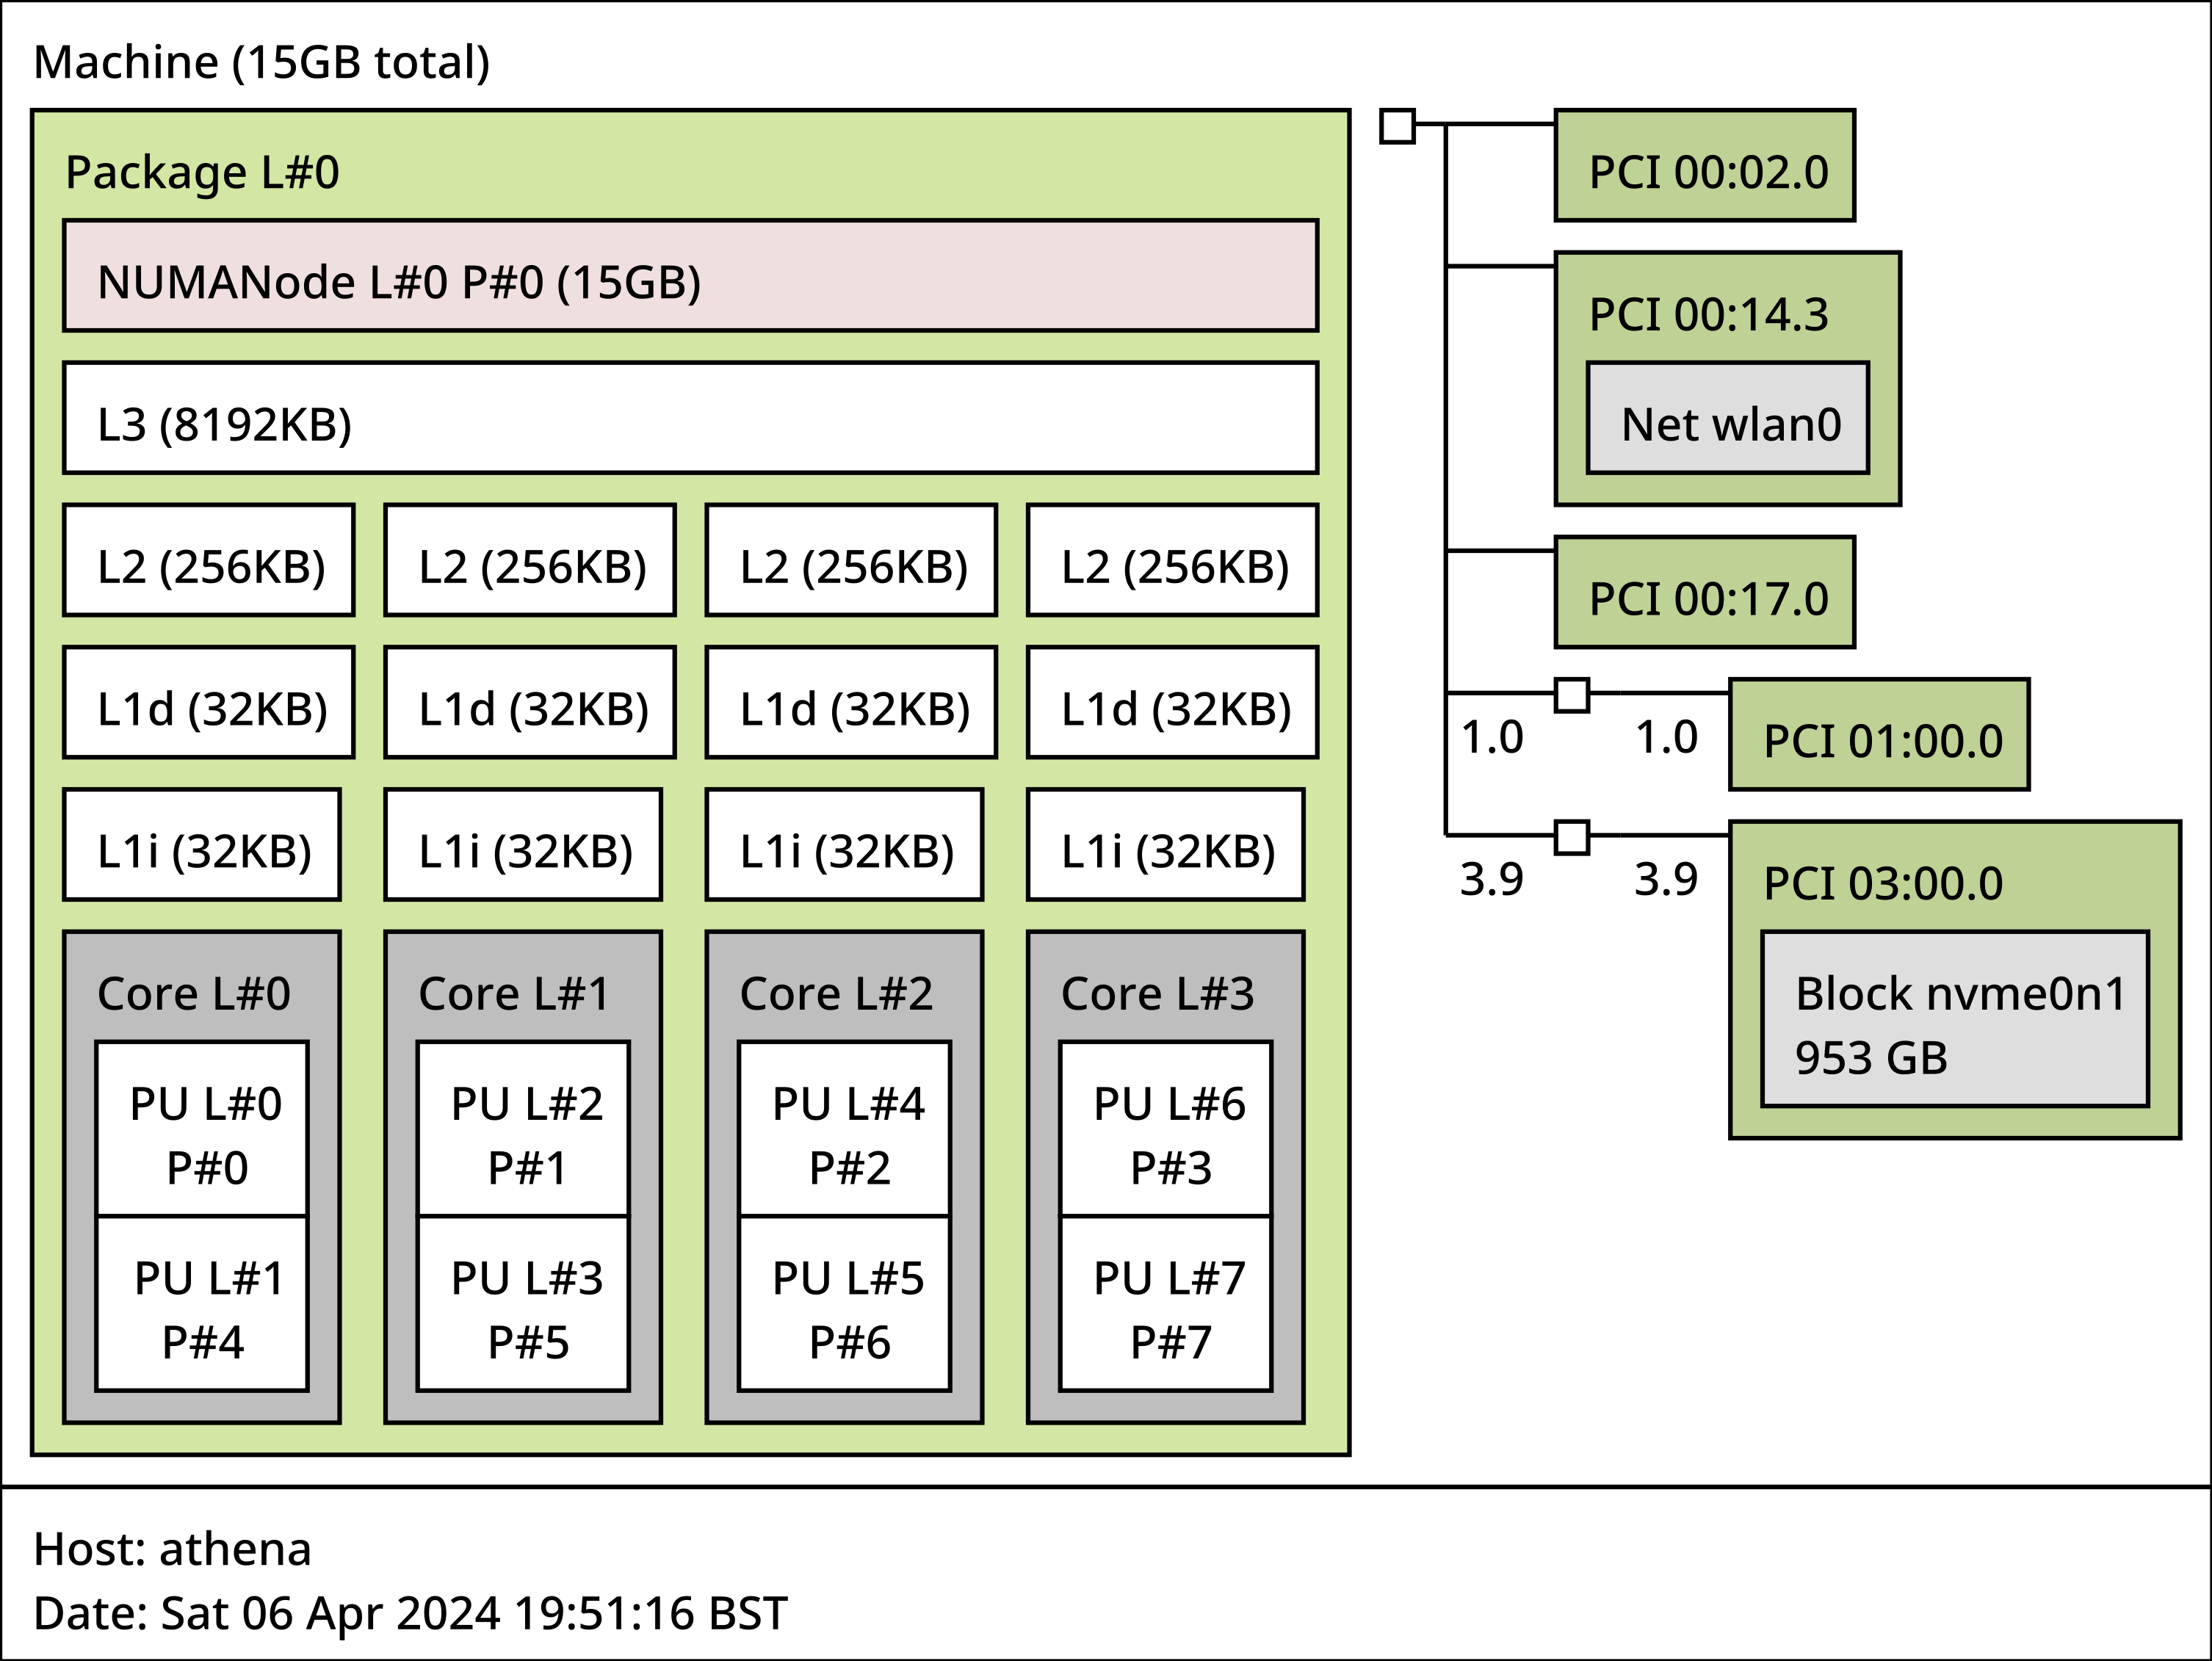
\includegraphics[width=0.75\textwidth]{images/8_appendix/athena-topology.png}
    \caption{Hardware topology of the Athena compute resource.}
    \label{fig:athena-topology}
\end{figure}

\begin{figure}[H]
    \centering
    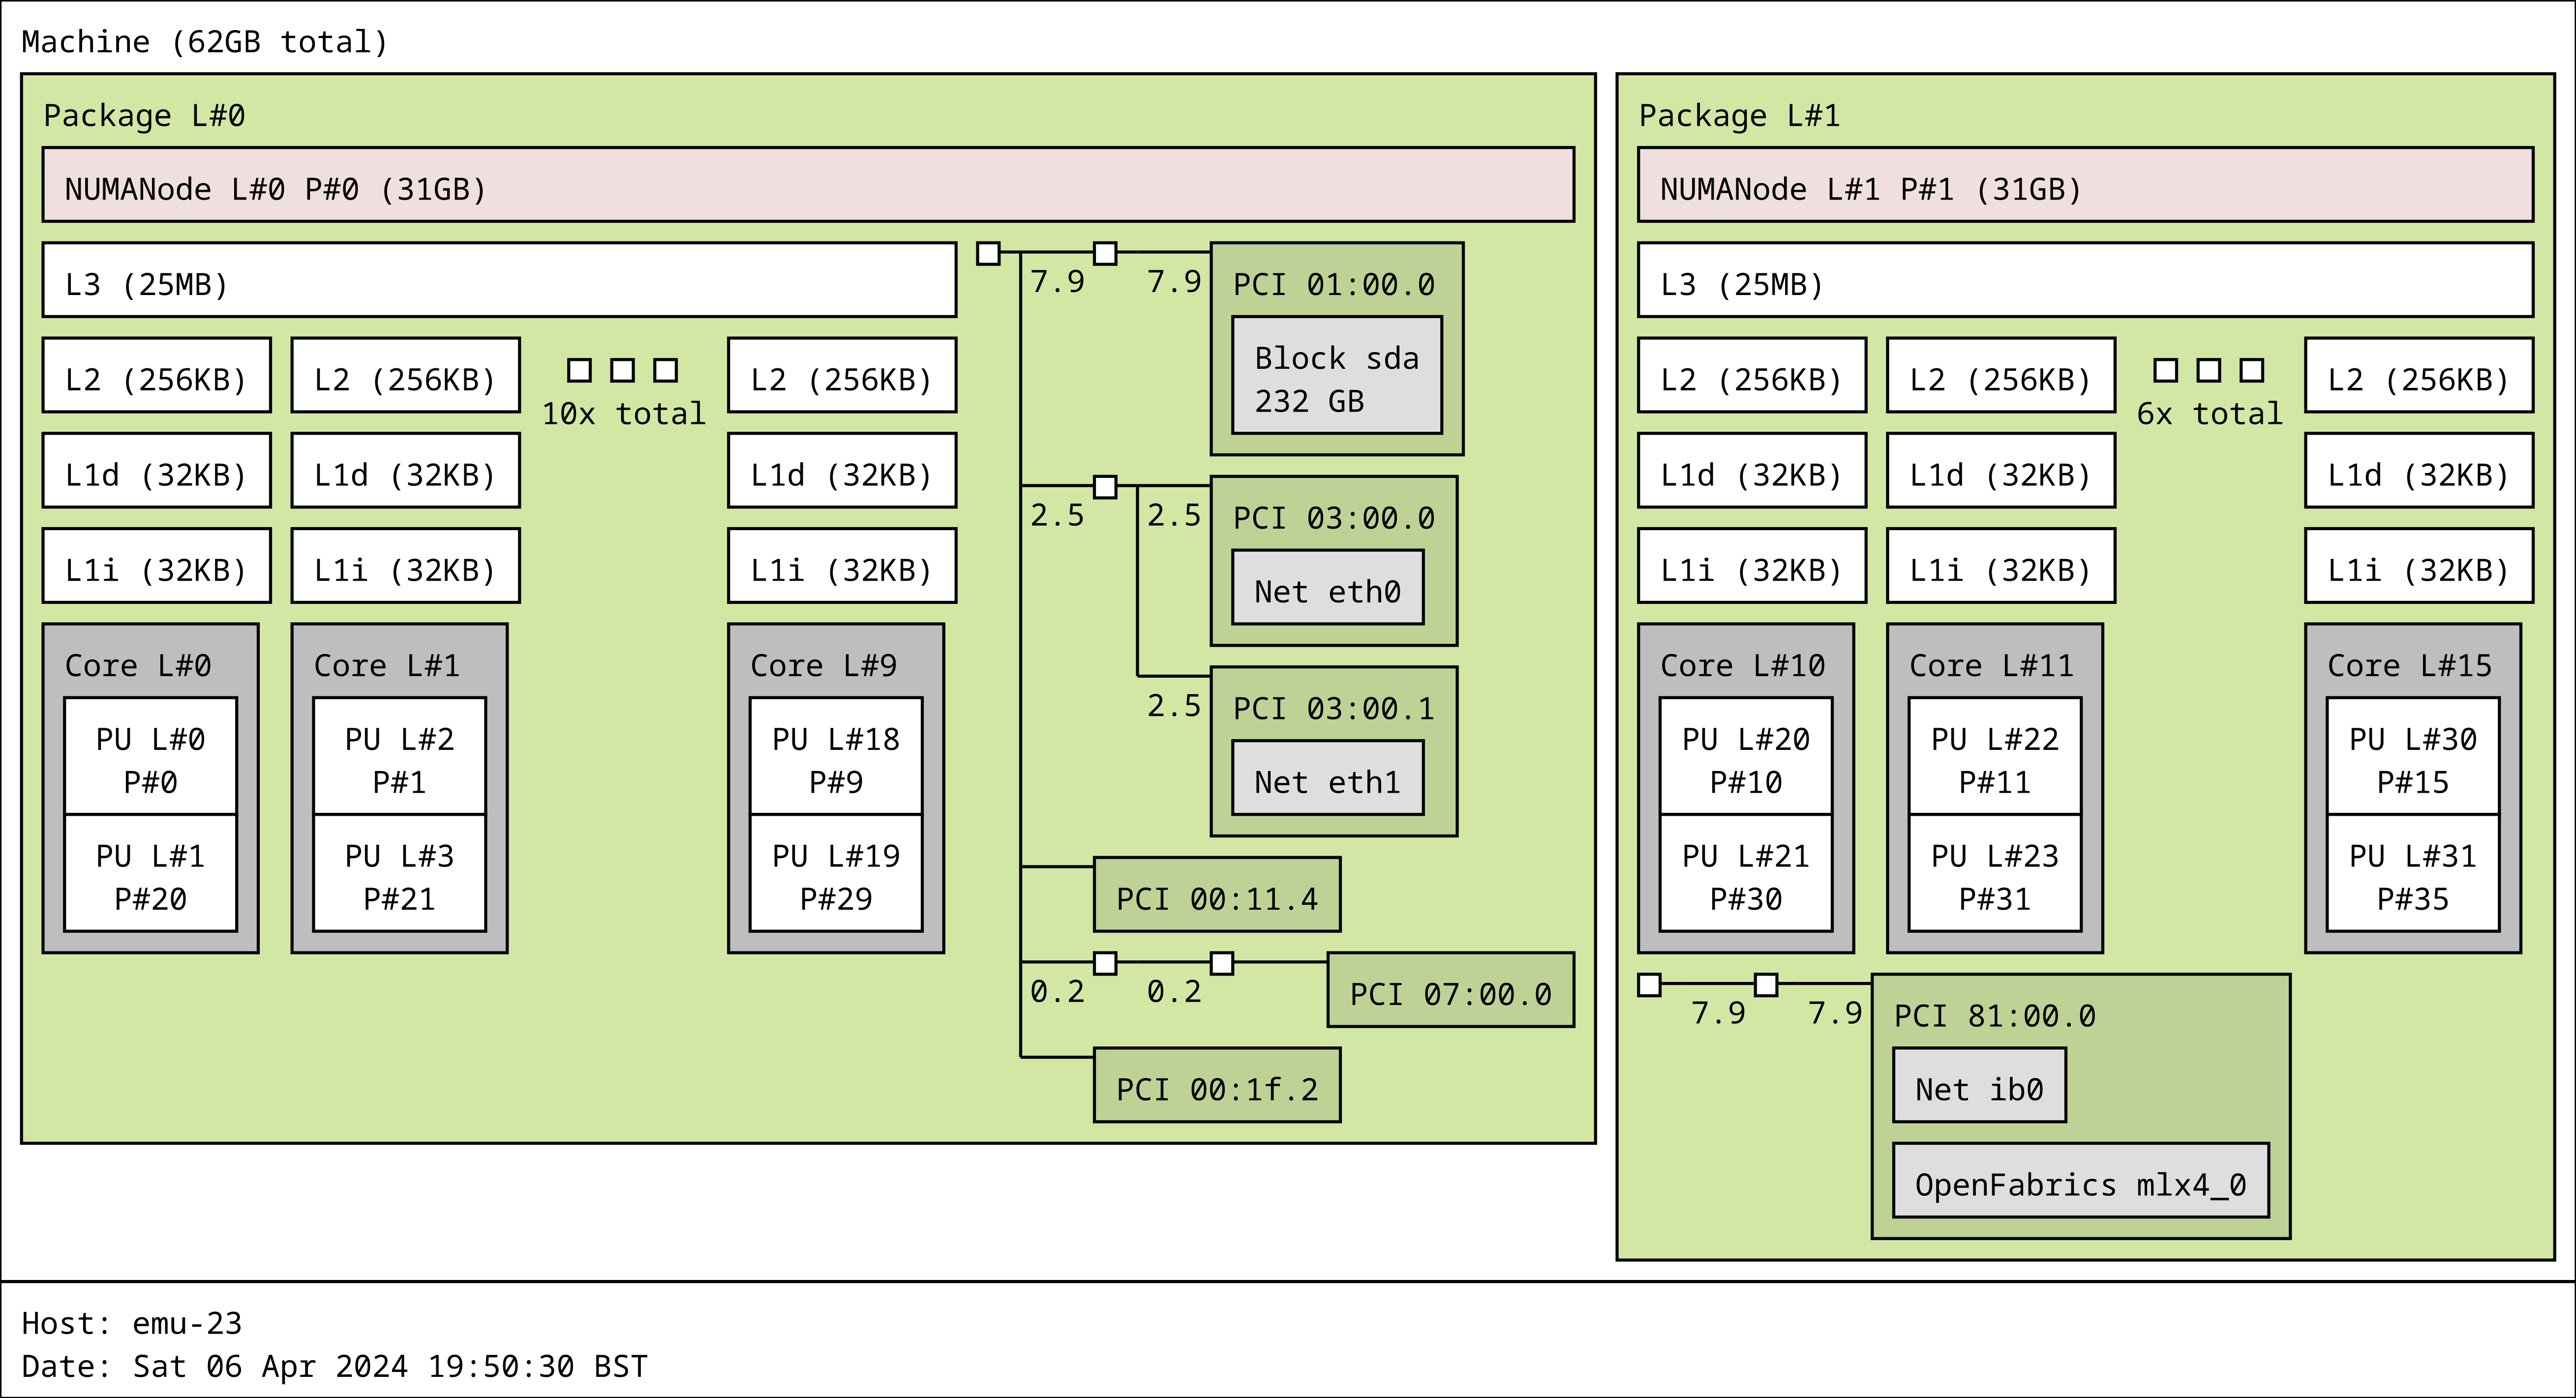
\includegraphics[width=0.85\textwidth]{images/8_appendix/kudu-topology.png}
    \caption{Hardware topology of the Kudu compute resource.}
    \label{fig:kudu-topology}
\end{figure}

\begin{figure}[H]
    \centering
    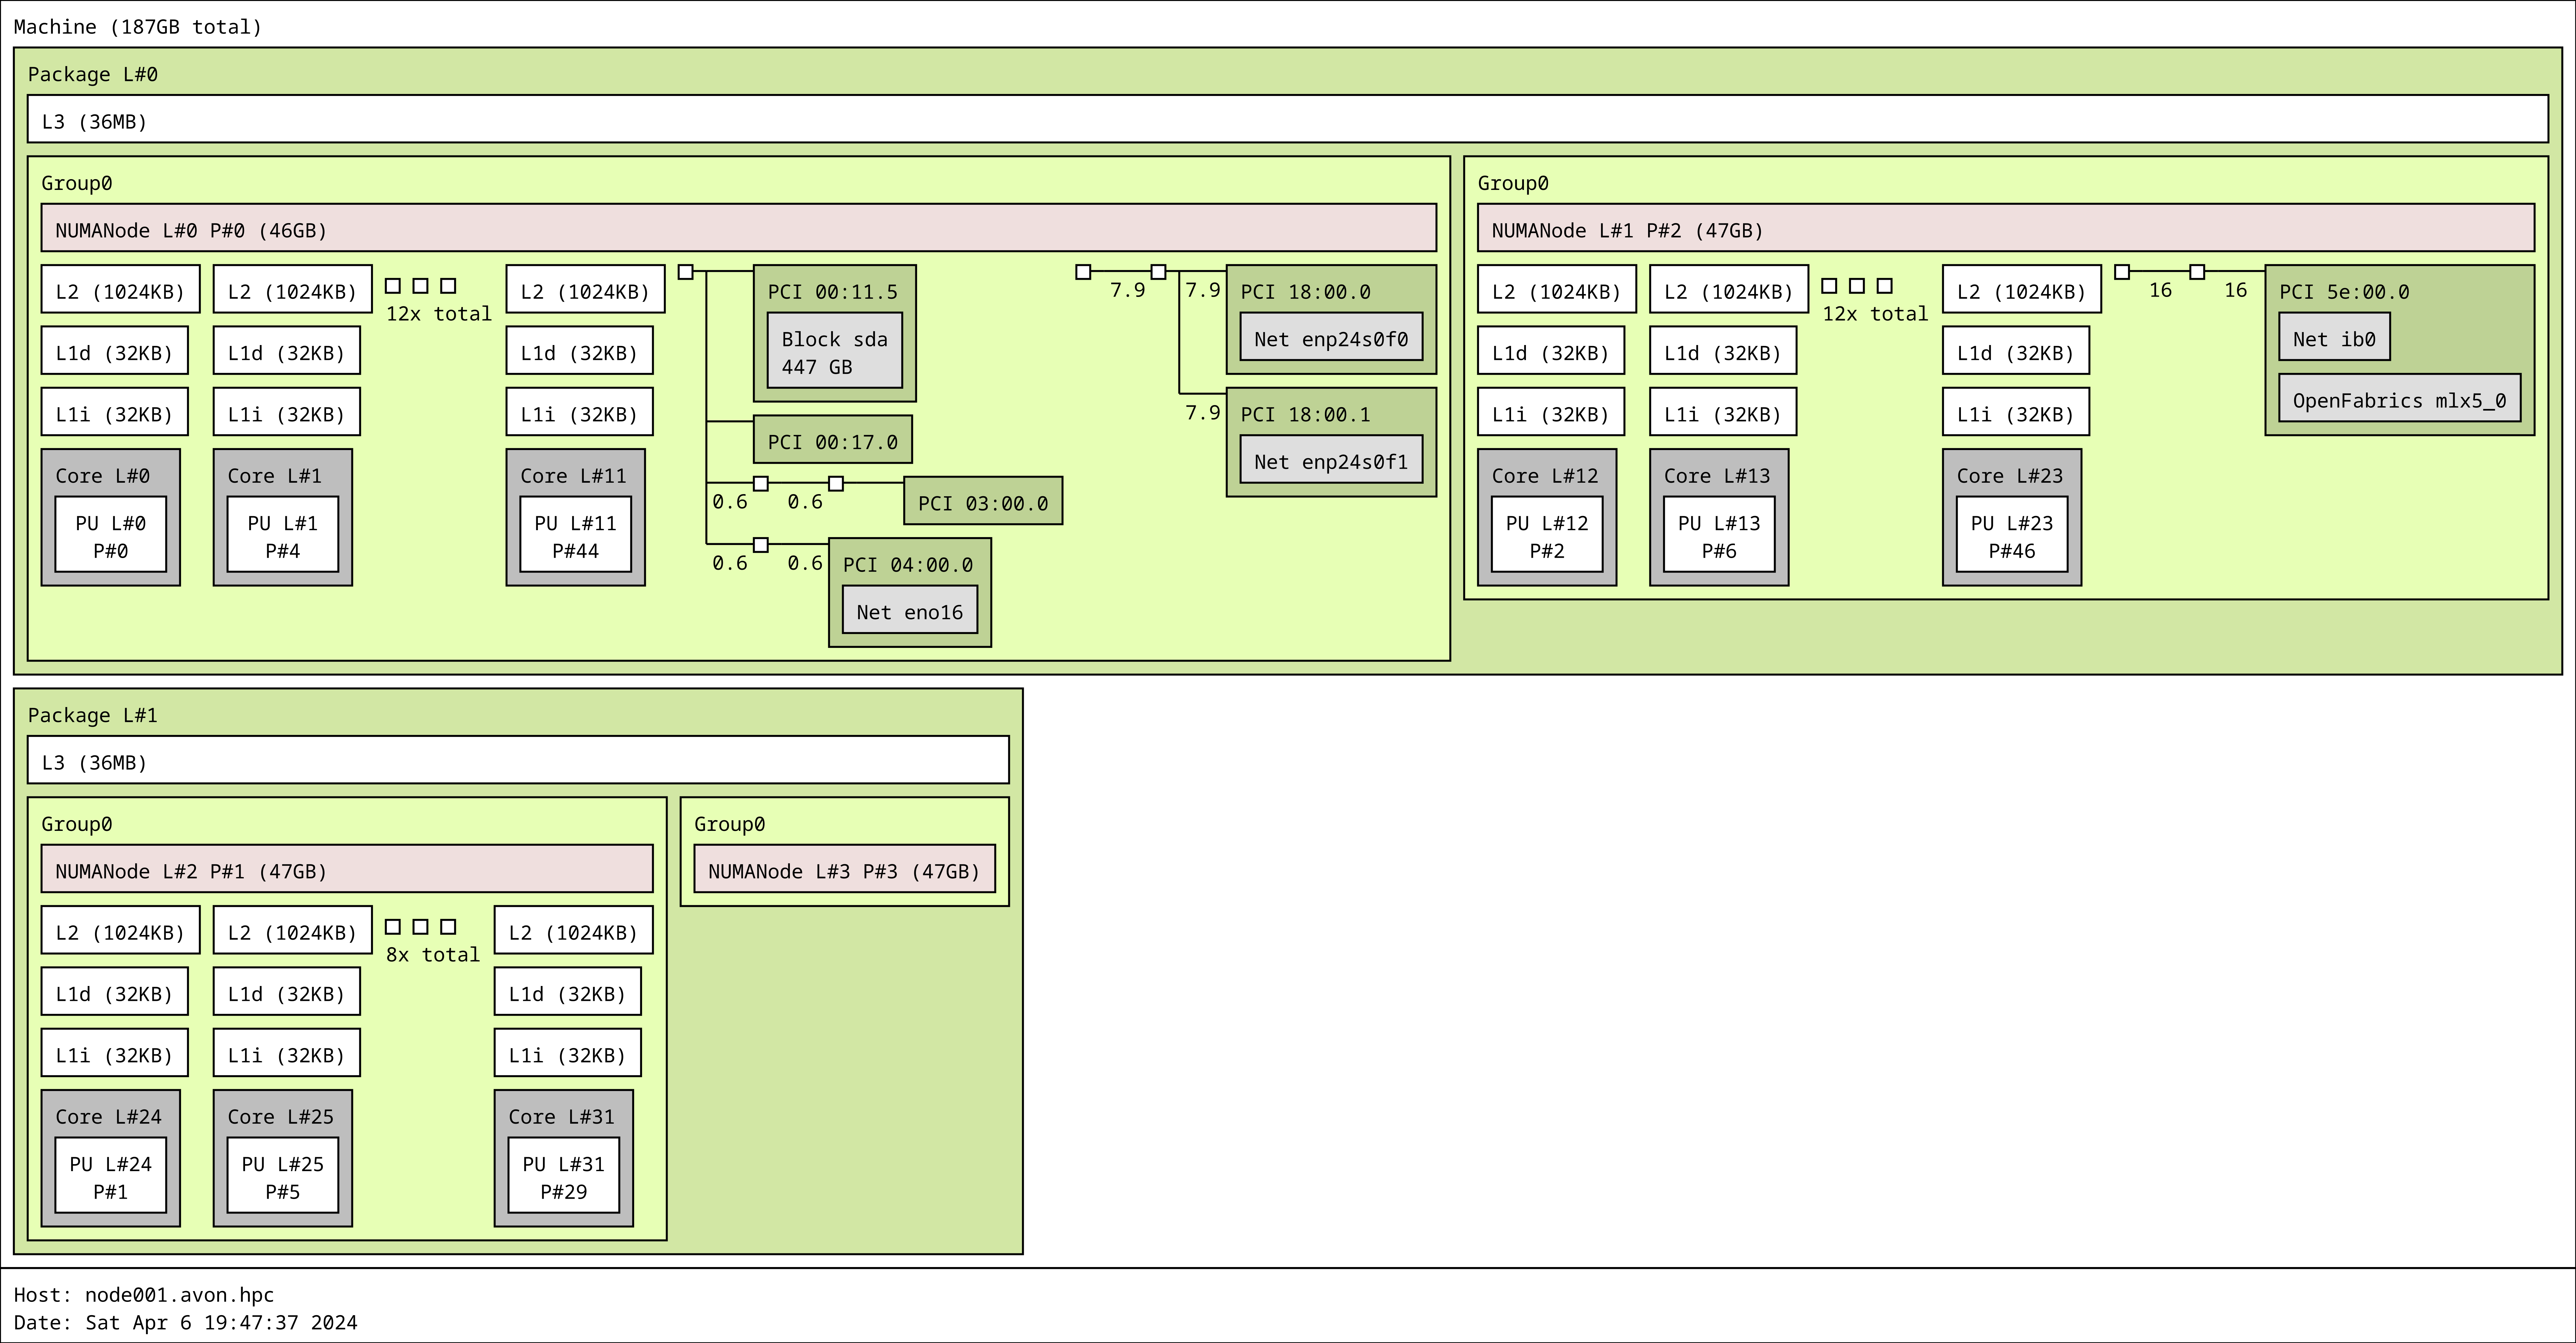
\includegraphics[width=0.95\textwidth]{images/8_appendix/avon-topology.png}
    \caption{Hardware topology of the Avon compute resource.}
    \label{fig:avon-topology}
\end{figure}

The results of running \texttt{lscpu} on the compute nodes for each of the systems are shown below in Listings \ref{listing:athena-lscpu}, \ref{listing:kudu-lscpu}, and \ref{listing:avon-lscpu}.

\begin{code}
    \begin{minted}{text}
Architecture:             x86_64
  CPU op-mode(s):         32-bit, 64-bit
  Address sizes:          39 bits physical, 48 bits virtual
  Byte Order:             Little Endian
CPU(s):                   8
  On-line CPU(s) list:    0-7
Vendor ID:                GenuineIntel
  Model name:             Intel(R) Core(TM) i7-8565U CPU @ 1.80GHz
    CPU family:           6
    Model:                142
    Thread(s) per core:   2
    Core(s) per socket:   4
    Socket(s):            1
    Stepping:             12
    CPU(s) scaling MHz:   21%
    CPU max MHz:          4600.0000
    CPU min MHz:          400.0000
    BogoMIPS:             4001.60
    Flags:                fpu vme de pse tsc msr pae mce cx8 apic sep mtrr pge mca cmov pat pse36 clflush dts acpi mmx fxsr sse sse2 ss ht tm pbe syscall nx pdpe1gb rdtscp lm constant_tsc art 
                          arch_perfmon pebs bts rep_good nopl xtopology nonstop_tsc cpuid aperfmperf pni pclmulqdq dtes64 monitor ds_cpl vmx est tm2 ssse3 sdbg fma cx16 xtpr pdcm pcid sse4_1 s
                          se4_2 x2apic movbe popcnt tsc_deadline_timer aes xsave avx f16c rdrand lahf_lm abm 3dnowprefetch cpuid_fault epb ssbd ibrs ibpb stibp ibrs_enhanced tpr_shadow flexpri
                          ority ept vpid ept_ad fsgsbase tsc_adjust sgx bmi1 avx2 smep bmi2 erms invpcid mpx rdseed adx smap clflushopt intel_pt xsaveopt xsavec xgetbv1 xsaves dtherm ida arat 
                          pln pts hwp hwp_notify hwp_act_window hwp_epp vnmi md_clear flush_l1d arch_capabilities
Virtualization features:  
  Virtualization:         VT-x
Caches (sum of all):      
  L1d:                    128 KiB (4 instances)
  L1i:                    128 KiB (4 instances)
  L2:                     1 MiB (4 instances)
  L3:                     8 MiB (1 instance)
NUMA:                     
  NUMA node(s):           1
  NUMA node0 CPU(s):      0-7
Vulnerabilities:          
  Gather data sampling:   Mitigation; Microcode
  Itlb multihit:          KVM: Mitigation: VMX disabled
  L1tf:                   Not affected
  Mds:                    Not affected
  Meltdown:               Not affected
  Mmio stale data:        Mitigation; Clear CPU buffers; SMT vulnerable
  Reg file data sampling: Not affected
  Retbleed:               Mitigation; Enhanced IBRS
  Spec rstack overflow:   Not affected
  Spec store bypass:      Mitigation; Speculative Store Bypass disabled via prctl
  Spectre v1:             Mitigation; usercopy/swapgs barriers and __user pointer sanitization
  Spectre v2:             Mitigation; Enhanced / Automatic IBRS, IBPB conditional, RSB filling, PBRSB-eIBRS SW sequence
  Srbds:                  Mitigation; Microcode
  Tsx async abort:        Not affected
    \end{minted}
    \caption{Output of the \texttt{lscpu} command on Athena.}
    \label{listing:athena-lscpu}
\end{code}

\begin{code}
    \begin{minted}{text}
Architecture:        x86_64
CPU op-mode(s):      32-bit, 64-bit
Byte Order:          Little Endian
CPU(s):              40
On-line CPU(s) list: 0-39
Thread(s) per core:  2
Core(s) per socket:  10
Socket(s):           2
NUMA node(s):        2
Vendor ID:           GenuineIntel
CPU family:          6
Model:               63
Model name:          Intel(R) Xeon(R) CPU E5-2660 v3 @ 2.60GHz
Stepping:            2
CPU MHz:             3300.000
CPU max MHz:         3300.0000
CPU min MHz:         1200.0000
BogoMIPS:            5199.67
Virtualization:      VT-x
L1d cache:           32K
L1i cache:           32K
L2 cache:            256K
L3 cache:            25600K
NUMA node0 CPU(s):   0-9,20-29
NUMA node1 CPU(s):   10-19,30-39
Flags:               fpu vme de pse tsc msr pae mce cx8 apic sep mtrr pge mca cmov pat pse36 clflush dts acpi mmx fxsr sse sse2 ss ht tm pbe syscall nx pdpe1gb rdtscp lm constant_tsc arch_perfmon pebs bts rep_good nopl xtopology nonstop_tsc cpuid aperfmperf pni pclmulqdq dtes64 monitor ds_cpl vmx smx est tm2 ssse3 sdbg fma cx16 xtpr pdcm pcid dca sse4_1 sse4_2 x2apic movbe popcnt tsc_deadline_timer aes xsave avx f16c rdrand lahf_lm abm cpuid_fault epb invpcid_single pti intel_ppin ssbd ibrs ibpb stibp tpr_shadow vnmi flexpriority ept vpid ept_ad fsgsbase tsc_adjust bmi1 avx2 smep bmi2 erms invpcid cqm xsaveopt cqm_llc cqm_occup_llc dtherm ida arat pln pts md_clear flush_l1d
    \end{minted}
    \caption{Output of the \texttt{lscpu} command on the Kudu compute node.}
    \label{listing:kudu-lscpu}
\end{code}

\begin{code}
    \begin{minted}{text}
Architecture:        x86_64
CPU op-mode(s):      32-bit, 64-bit
Byte Order:          Little Endian
CPU(s):              48
On-line CPU(s) list: 0-47
Thread(s) per core:  1
Core(s) per socket:  24
Socket(s):           2
NUMA node(s):        4
Vendor ID:           GenuineIntel
CPU family:          6
Model:               85
Model name:          Intel(R) Xeon(R) Platinum 8268 CPU @ 2.90GHz
Stepping:            7
CPU MHz:             3506.916
BogoMIPS:            5800.00
Virtualization:      VT-x
L1d cache:           32K
L1i cache:           32K
L2 cache:            1024K
L3 cache:            36608K
NUMA node0 CPU(s):   0,4,8,12,16,20,24,28,32,36,40,44
NUMA node1 CPU(s):   1,5,9,13,17,21,25,29,33,37,41,45
NUMA node2 CPU(s):   2,6,10,14,18,22,26,30,34,38,42,46
NUMA node3 CPU(s):   3,7,11,15,19,23,27,31,35,39,43,47
Flags:               fpu vme de pse tsc msr pae mce cx8 apic sep mtrr pge mca cmov pat pse36 clflush dts acpi mmx fxsr sse sse2 ss ht tm pbe syscall nx pdpe1gb rdtscp lm constant_tsc art arch_perfmon pebs bts rep_good nopl xtopology nonstop_tsc cpuid aperfmperf pni pclmulqdq dtes64 monitor ds_cpl vmx smx est tm2 ssse3 sdbg fma cx16 xtpr pdcm pcid dca sse4_1 sse4_2 x2apic movbe popcnt tsc_deadline_timer aes xsave avx f16c rdrand lahf_lm abm 3dnowprefetch cpuid_fault epb cat_l3 cdp_l3 invpcid_single intel_ppin ssbd mba ibrs ibpb stibp ibrs_enhanced fsgsbase tsc_adjust bmi1 hle avx2 smep bmi2 erms invpcid cqm mpx rdt_a avx512f avx512dq rdseed adx smap clflushopt clwb intel_pt avx512cd avx512bw avx512vl xsaveopt xsavec xgetbv1 xsaves cqm_llc cqm_occup_llc cqm_mbm_total cqm_mbm_local dtherm ida arat pln pts pku ospke avx512_vnni md_clear flush_l1d arch_capabilities
    \end{minted}
    \caption{Output of the \texttt{lscpu} command on Athena.}
    \label{listing:avon-lscpu}
\end{code}

\chapter{Open source work}
\label{ch:open-source-appendix}

\section{\texttt{autocxx} pull request}
\label{sec:autocxx-pull-request-appendix}

\begin{figure}[H]
    \centering
    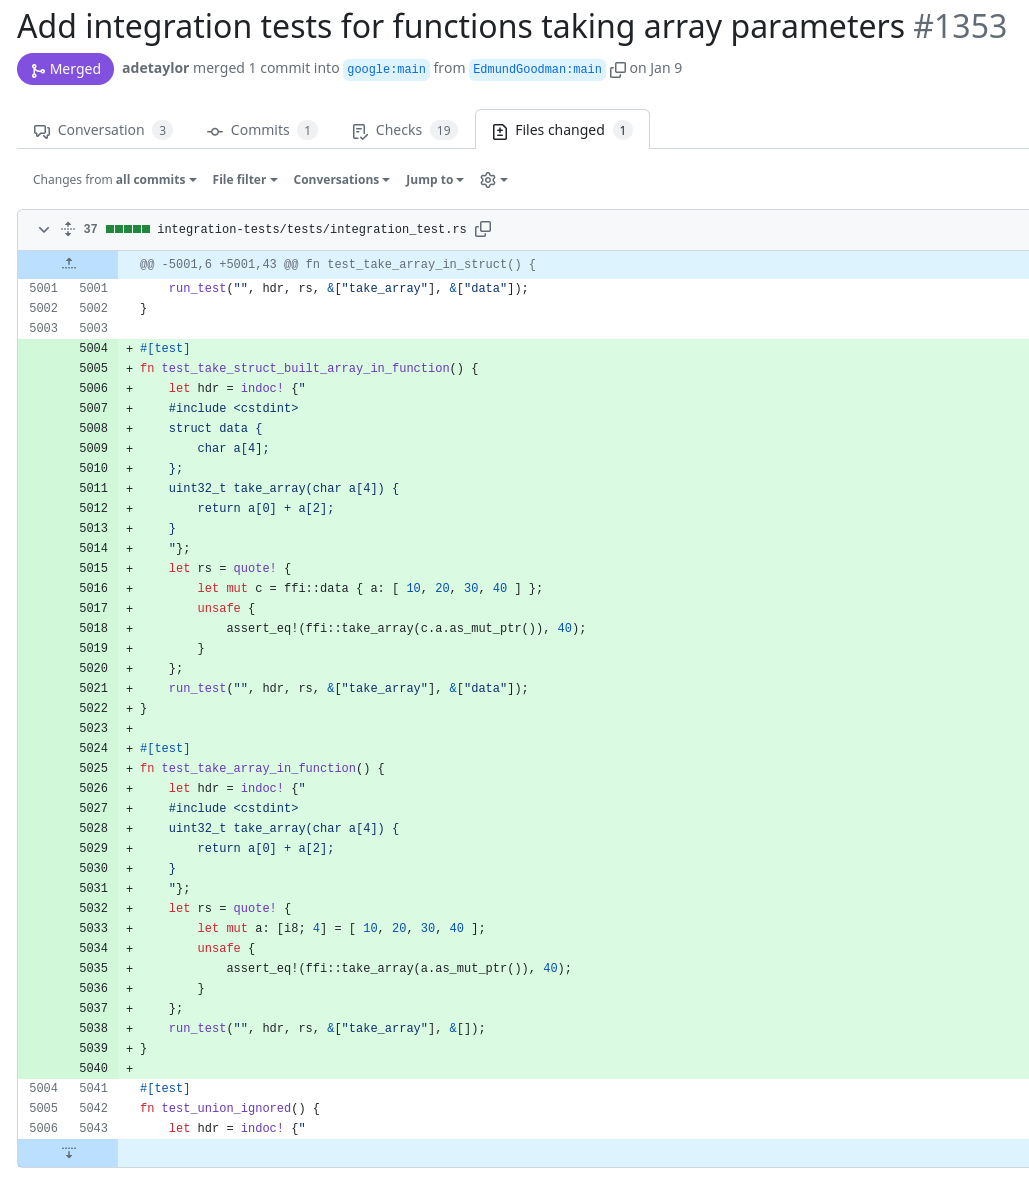
\includegraphics[width=\textwidth]{images/8_appendix/autocxx_pr.png}
    \caption{Screenshot of the pull request adding integration tests for array support made into \texttt{autocxx}.}
    \label{fig:autocxx_pr}
\end{figure}